\documentclass{article}
\usepackage[a4paper, margin=2.5cm]{geometry}
\usepackage{Csharp}
\usepackage[ngerman]{babel}
\lstset{
	basicstyle=\tiny
}

\usepackage{graphicx,capt-of}
\graphicspath{ {images/} }

\begin{document}

\title{
{\Huge Aufgabe 5\\Widerstand}\\
\vspace{.5cm}
\begin{large}
Team-Name: Bruteforce\\
Team-ID: 00139\\
Bearbeiter:\\ 
\end{large}
\begin{normalsize}
P1,
P3,
P4,
P2
\end{normalsize}
}
\author{}
\date{}
\maketitle
\vspace{5cm}
\tableofcontents
\listoffigures
\lstlistoflistings
\newpage
\flushleft

\section{Widerstand}

\subsection{Lösungsansatz}
Für die Lösung des Problems haben wir uns für einen Bruteforce-Algorithmus mit Backtracking entschieden, das heißt wir bauen einen Baum aller Möglichkeiten auf, bauen jedoch nie an einem Ast davon weiter, sollte die Differenz zum Zielwiderstand jemals nicht das aktuelle Top-Ergebnis sein.
Dieser Ansatz erlaubt eine (relativ) kompakte Implementierung durch Rekursion und bietet trotzdem eine (relativ) schnelle Lösung.

\subsection{Implementierung}
\subsubsection{Datenmodellierung}
Zur Implementierung des Algorithmus haben wir uns wie bei vorherigen Aufgaben für eine objekt-orientierte Lösung in C\# entschieden, welches die Datenmodellierung stark erleichtert.
Zur Datenmodellierung haben wir 3 Klassen für Widerstände definiert, die alle ein gemeinsames Interface $IResistor$ (siehe Listing \ref{LIS:IRes} auf Seite \pageref{LIS:IRes}) implementieren. Dieses Interface enthält den Gesamtwiderstand und eine Liste der enthaltenen Widerstände. Weiterdem enthält das Interface die Menge an enthaltenen Widerständen, welche die Summe der selben Eigenschaft der Widerständen in der Widerstands-Liste ist. Letzlich enthält das Interface eine Methode $Draw(style)$, welche für das Zeichnen der Resistoren verantwortlich ist. Die 3 Klassen die dieses Interface implementieren sind ein normaler Widerstand (Listing \ref{LIS:Single} auf Seite \pageref{LIS:Single}),  und zwei Komposit-Widerstände, der parallelele (Listing \ref{LIS:Par} auf Seite \pageref{LIS:Par}) und serielle (Listing \ref{LIS:Serial} auf Seite \pageref{LIS:Serial}) Widerstand.

\subsubsection{Algorithmus}
Der eigentliche Algorithmus besteht aus einer Mischung von Rekursion und Iteration.
Die Hauptmethode $BuildResistor(targetResistance,\;resistor,\;maxResistorCount,\;availableResistors)$ nimmt den Zielwiderstand, den aktuellen Komposit-Widerstand, die maximale erlaubte Menge an erlaubten Widerständen (k) und eine Liste aller zur Verfügung stehenden Widerstände. Die Methode ermittelt zuerst die kleinste Differenz zum Ziel-Widerstand und alle Komposit-Widerstände die in dem übergebenen Komposit-Widerstand enthalten sind.
Daraufhin iteriert das Programm über diese einzelnen Komposit-Widerstände und nimmt einen Widerstand aus der Liste verfügbarer Widerstände, welchen es daraufhin in den aktuellen Komposit-Widerstand einfügt, oder es selektiert einen zweiten verfügbaren Widerstand und fügt einen parallelen/seriellen Widerstand bestehend aus beiden ausgewählten an. Sollte die Differenz die kleinste bisher erreichte Differenz zum Ziel-Widerstand unterschreiten wird die $BuildResistor$-Methode rekursiv aufgerufen. Sollte die Differenz 0 betragen wird die maximale Menge an Resistoren für den gesamten Baum auf die Menge an Widerständen im aktuellen Komposit-Widerstand gesetzt. Sollte keine dieser beiden Bedingungen zutreffen so wird keine Aktion vorgenommen.
Sollte die Anzahl an Widerständen im aktuellen Komposit-Widerstand jemals die maximale Menge an Widerständen überschreiten stoppt die Methode und geht zurück im Baum.

\subsection{Graphische Darstellung}
Zur graphischen Darstellung der Widerstände implementieren die 3 Widerstands-Klassen die Methode $Draw(style)$, welche bei einzelnen Widerständen eine Box mit dem Widerstand als Aufschrift ausgibt, und bei seriellen und parallelen Widerständen eine Aufreihung der Ergebnisse der $Draw$ Methode seiner enthaltenen Widerstände ausgibt.

\newpage
\subsection{Beispiel}
\begin{center}
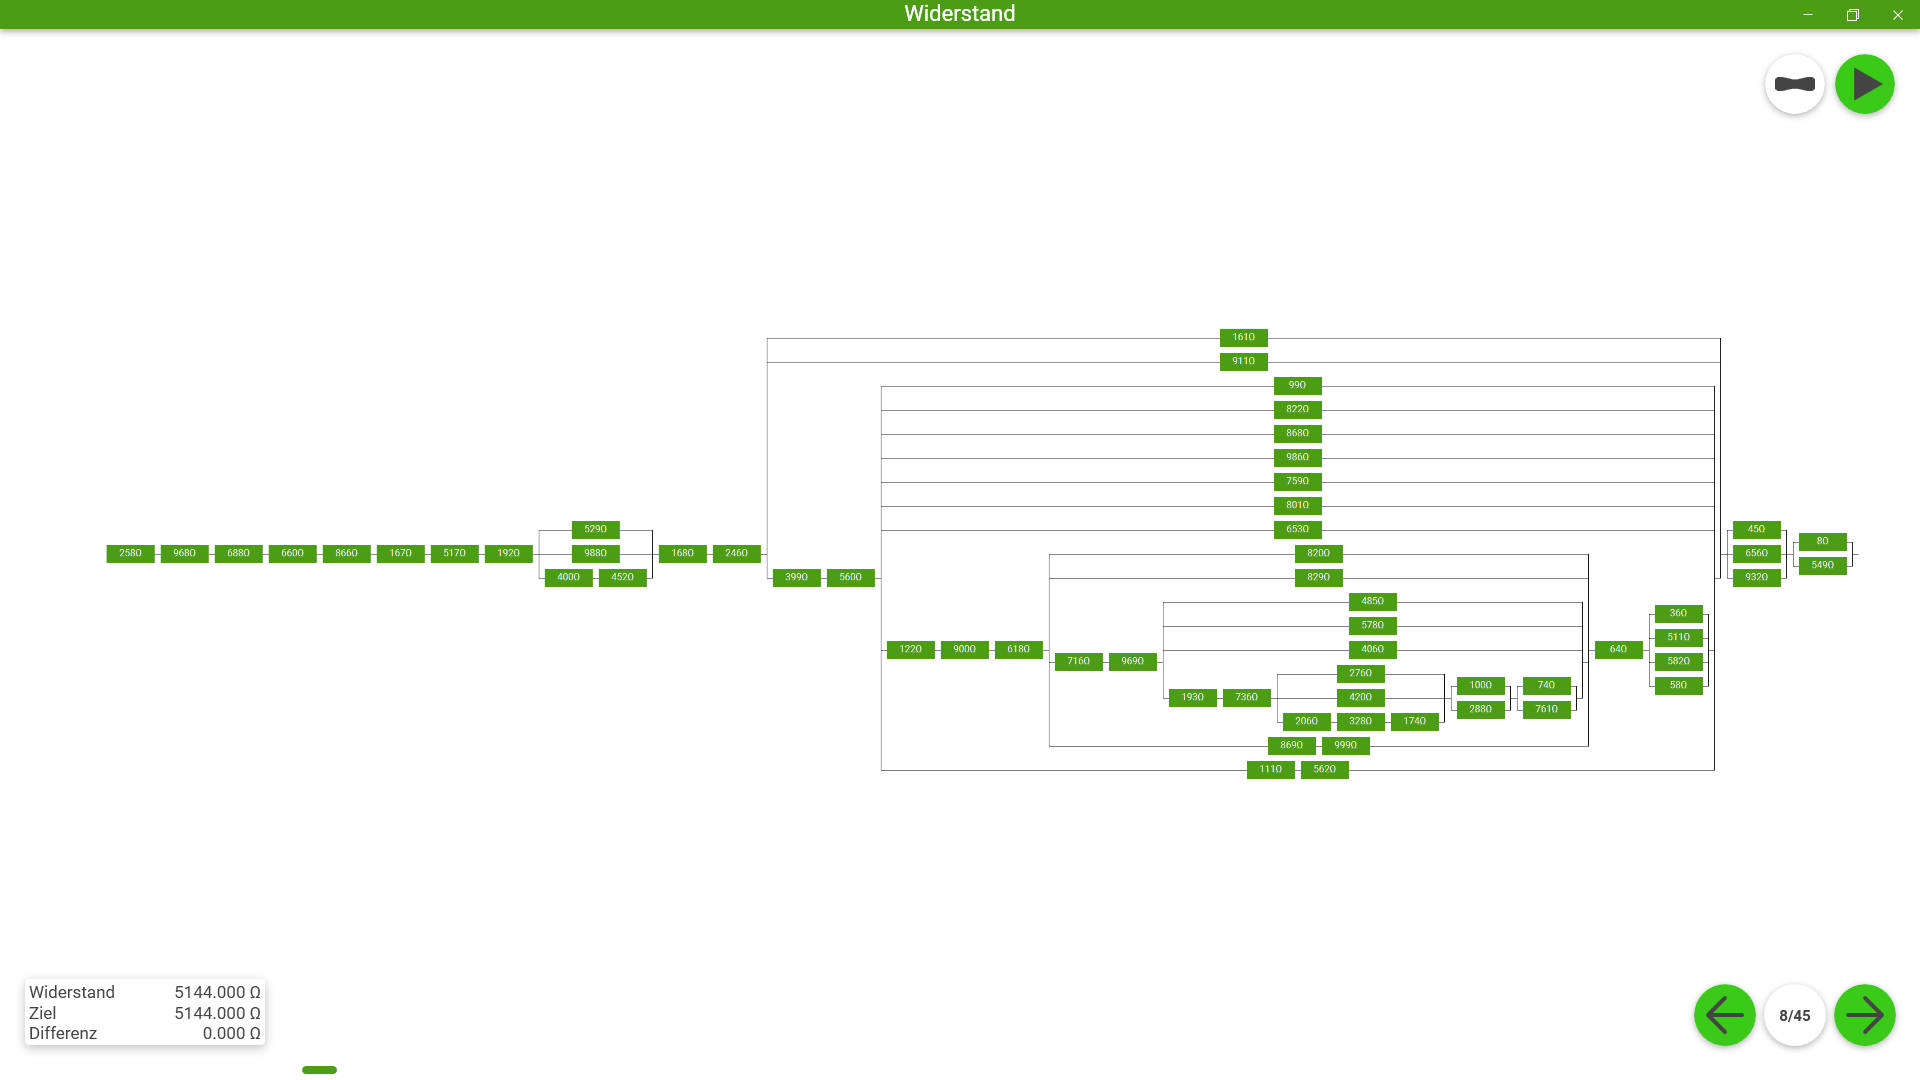
\includegraphics[scale=.3]{images/widerstand}
\captionof{figure}{100 zufällige Widerstände, 60 maximal erlaubt, 5144.0 Ohm Ziel-Widerstand}
\label{FIG:widerstand}
\end{center}


\subsection{Code}
\begin{Csharp}[caption=Interface IResistor,label=LIS:IRes]
public interface IResistor : ICloneable
{
    double Value { get; }
    List<IResistor> Resistors { get; set; }
    int Count { get; }

    Bitmap Draw(ResistorStyle style);
}

public struct ResistorStyle
{
    public Color ResistorColor, WireColor, TextColor, BackColor;
    public string Font;

    public int ResistorWidth, ResistorHeight;
    public int WireLength, WireThickness;
}
\end{Csharp}

\begin{Csharp}[caption=Klasse SingleResistor,label=LIS:Single] 
public class SingleResistor : IResistor
{
    public SingleResistor() { }

    public SingleResistor(double val)
    {
        Value = val;
    }

    public double Value { get; set; }
    public List<IResistor> Resistors
    {
        get => throw new Exception("Resistors don't have Resistors");
        set => throw new Exception("Resistors don't have Resistors");
    }

    public int Count => 1;
    public int Width => 1;
    public int Height => 1;

    public static implicit operator SingleResistor(double val) => new SingleResistor(val);

    public object Clone() => new SingleResistor { Value = Value };
    
    public Bitmap Draw(ResistorStyle style)
    {
        string value = Value.ToString(CultureInfo.InvariantCulture) + " Ohm";
        Bitmap bitmap = new Bitmap(style.ResistorWidth, style.ResistorHeight, PixelFormat.Format32bppArgb);

        using (Graphics g = Graphics.FromImage(bitmap))
        {
            g.FillRectangle(new SolidBrush(style.BackColor), 0, 0, bitmap.Width, bitmap.Height);

            g.FillRectangle(new SolidBrush(style.ResistorColor), 0, 0, bitmap.Width - style.WireLength, bitmap.Height);
            g.DrawString(value, new Font(style.Font, bitmap.Height / 2 - 3), new SolidBrush(style.TextColor), (bitmap.Width - style.WireLength) / 2, bitmap.Height / 2, new StringFormat
            {
                LineAlignment = StringAlignment.Center,
                Alignment = StringAlignment.Center
            });
            g.DrawLine(new Pen(new SolidBrush(style.WireColor), style.WireThickness), bitmap.Width - style.WireLength, bitmap.Height / 2, bitmap.Width, bitmap.Height / 2);
        }

        return bitmap;
    }
}
\end{Csharp}

\begin{Csharp}[caption=Klasse SerialResistor,label=LIS:Serial] 
public class SerialResistor : IResistor
{
    public SerialResistor()
    {
        Resistors = new List<IResistor>();
    }

    public SerialResistor(params double[] val)
    {
        Resistors = new List<IResistor>(val.Select(x => (SingleResistor)x));
    }

    public SerialResistor(params IResistor[] val)
    {
        Resistors = val.ToList();
    }

    public List<IResistor> Resistors { get; set; }
    public double Value  => Resistors.Sum(x => x.Value);

    public int Count => Resistors.Sum(x => x.Count);

    public object Clone() => new SerialResistor { Resistors = Resistors.Select(x => (IResistor)x.Clone()).ToList() };

    public Bitmap Draw(ResistorStyle style)
    {
        List<Bitmap> resistors = Resistors.Select(x => x.Draw(style)).ToList();

        Bitmap bitmap = new Bitmap(resistors.Sum(x => x.Width), resistors.Max(x => x.Height), PixelFormat.Format32bppArgb);

        using (Graphics g = Graphics.FromImage(bitmap))
        {
            g.FillRectangle(new SolidBrush(style.BackColor), 0, 0, bitmap.Width, bitmap.Height);

            int sum = 0;

            resistors.ForEach(res =>
            {
                g.DrawImage(res, sum, (bitmap.Height - res.Height) / 2);
                sum += res.Width;
            });
        }

        return bitmap;
    }
}
\end{Csharp}

\begin{Csharp}[caption=Klasse ParallelResistor,label=LIS:Par] 
public class ParallelResistor : IResistor
{
    public ParallelResistor()
    {
        Resistors = new List<IResistor>();
    }

    public ParallelResistor(params double[] val)
    {
        Resistors = new List<IResistor>(val.Select(x => (SingleResistor)x));
    }

    public ParallelResistor(params IResistor[] val)
    {
        Resistors = new List<IResistor>(val.Select(x => x));
    }

    public List<IResistor> Resistors { get; set; }
    public double Value => 1f / Resistors.Sum(x => 1f / x.Value);

    public int Count => Resistors.Sum(x => x.Count);

    public object Clone() => new ParallelResistor { Resistors = Resistors.Select(x => (IResistor)x.Clone()).ToList() };

    public Bitmap Draw(ResistorStyle style)
    {
        List<Bitmap> resistors = Resistors.Select(x => x.Draw(style)).ToList();

        Bitmap bitmap = new Bitmap(resistors.Max(x => x.Width) + style.WireLength * 2, resistors.Sum(x => x.Height + style.WireLength) - style.WireLength, PixelFormat.Format32bppArgb);

        using (Graphics g = Graphics.FromImage(bitmap))
        {
            g.FillRectangle(new SolidBrush(style.BackColor), 0, 0, bitmap.Width, bitmap.Height);

            int sum = 0;

            Pen pen = new Pen(new SolidBrush(style.WireColor), style.WireThickness);

            resistors.ForEach(res =>
            {
                g.DrawLine(pen, 0, sum + res.Height / 2, bitmap.Width - style.WireLength - style.WireThickness, sum + res.Height / 2);
                g.DrawImage(res, (bitmap.Width - res.Width) / 2, sum);
                sum += res.Height + style.WireLength;
            });

            g.DrawLine(pen, 0, resistors[0].Height / 2, 0, sum - style.WireLength - resistors.Last().Height / 2);
            g.DrawLine(pen, bitmap.Width - style.WireLength - style.WireThickness, resistors[0].Height / 2, bitmap.Width - style.WireLength - style.WireThickness, sum - style.WireLength - resistors.Last().Height / 2);
            g.DrawLine(pen, bitmap.Width - style.WireThickness, bitmap.Height / 2, bitmap.Width - style.WireLength - style.WireThickness, sum - style.WireLength - bitmap.Height / 2);
        }

        return bitmap;
    }
}
\end{Csharp}

\begin{Csharp}[caption=Klasse ResistorBuilder,label=LIS:Buildr] 
public static class ResistorBuilder
{
    public static List<IResistor> BuildResistor(double targetResistance, int k, List<double> resistors, Action<List<IResistor>, IResistor> callback = null)
    {
        return BuildResistor(targetResistance, null, null, ref k, resistors, callback);
    }
    private static List<IResistor> BuildResistor(double targetResistance, IResistor prev, List<IResistor> all, ref int k, List<double> resistors, Action<List<IResistor>, IResistor> callback = null)
    {
        if (all == null) all = new List<IResistor>();
        if (prev == null) prev = new SerialResistor();

        if (prev.Count >= k)
        {
            if (prev.Count == k) all.AddResistor(prev, targetResistance);
            return all;
        }

        IResistor resistor = (IResistor)prev.Clone();
        if (callback != null && (resistor is SingleResistor || resistor.Resistors.Count > 0)) callback(all, resistor);

        double bestResult = Math.Min(all.Count == 0 ? double.PositiveInfinity 
                                                    : all.Min(x => Math.Abs(x.Value - targetResistance)), Math.Abs(prev.Value - targetResistance));

        List<IResistor> content = new List<IResistor>();
        void RecurseResistors(IResistor res)
        {
            if (!(res is SingleResistor))
            {
                content.Add(res);
                res.Resistors.ForEach(RecurseResistors);
            }
        }

        RecurseResistors(resistor);
        content = content.Distinct().ToList();

        double RecurseOption(IResistor subResistor, IResistor newResistor, ref int remainingK)
        {
            subResistor.Resistors.Add(newResistor);
            Cleanup(ref newResistor);
            double diff = Math.Abs(resistor.Value - targetResistance);
            if (!all.Contains(resistor))
            {
                if (diff == 0)
                {
                    all.AddResistor((IResistor)resistor.Clone(), targetResistance);
                    remainingK = Math.Min(resistor.Count, remainingK);
                }
                else if (diff < bestResult)
                {
                    List<IResistor> results = BuildResistor(targetResistance, resistor, all, ref remainingK, new List<double>(resistors), callback);

                    if (results.Count == 0) all.AddResistor((IResistor)resistor.Clone(), targetResistance);
                    else all.AddResistors(results, targetResistance);

                    all = all.Distinct().ToList();
                }
            }
            subResistor.Resistors.RemoveAt(subResistor.Resistors.Count - 1);
            return diff;
        }

        foreach (IResistor subResistor in content)
        {
            for (int i = 0; i < resistors.Count; i++)
            {
                double resistance0 = resistors[i];
                resistors.RemoveAt(i);

                if (RecurseOption(subResistor, new SingleResistor(resistance0), ref k) == 0) goto Exit;

                for (int j = 0; j < resistors.Count; j++)
                {
                    double resistance1 = resistors[j];
                    resistors.RemoveAt(j);

                    if (RecurseOption(subResistor, new SerialResistor(resistance0, resistance1), ref k) == 0) goto Exit;
                    if (RecurseOption(subResistor, new ParallelResistor(resistance0, resistance1), ref k) == 0) goto Exit;

                    resistors.Add(resistance1);
                }

                resistors.Add(resistance0);
            }
        }

        Exit:

        return all;
    }

    public static void AddResistor(this List<IResistor> list, IResistor resistor, double targetResistance)
    {
        int i = 0;
        while (i < list.Count && Math.Abs(list[i].Value - targetResistance) < Math.Abs(resistor.Value - targetResistance)) i++;
        list.Insert(i, resistor);
    }

    public static void AddResistors(this List<IResistor> list, List<IResistor> resistors, double targetResistance)
    {
        resistors = new List<IResistor>(resistors);
        for (int i = 0; i < resistors.Count; i++)
        {
            list.AddResistor(resistors[i], targetResistance);
        }
    }

    public static void Cleanup(ref IResistor resistor)
    {
        if (!(resistor is SingleResistor))
        {
            if (resistor.Resistors.Count == 0)
            {
                throw new Exception("Invalid resistor");
            }
            else if (resistor.Resistors.Count == 1)
            {
                IResistor internalResistor = resistor.Resistors[0];
                Cleanup(ref internalResistor);
                resistor = internalResistor;
            }
            else
            {
                resistor.Resistors.ForEach(x => Cleanup(ref x));
                resistor.Resistors = resistor.Resistors.OrderBy(x => x.Value).ToList();
            }
        }
    }
}
\end{Csharp}


\end{document}